\documentclass[twoside,14pt,a4paper,notitlepage]{memoir}

\usepackage{xltxtra,fontspec,xunicode}
\defaultfontfeatures{Scale=MatchLowercase}
\setmainfont{CMU Sans Serif}

\usepackage[top=1.8cm,bottom=1.8cm,outer=1.8cm,inner=4.2cm]{geometry}

\usepackage{hyperref}
\hypersetup{
    colorlinks=true,       % false: boxed links; true: colored links
    linkcolor=black,          % color of internal links (change box color with linkbordercolor)
    citecolor=black,        % color of links to bibliography
    filecolor=blue,      % color of file links
    urlcolor=blue           % color of external links
}

%\usepackage{rotating}
\usepackage{pdfpages}
\usepackage[none]{hyphenat}
\usepackage{lipsum}

\makeatletter
\let\l@chapternonum\l@chapter
\newcounter{chapternonum}
\renewcommand{\thechapternonum}{}
\makeatother


\begin{document}
\pagestyle{plain}

% Poster
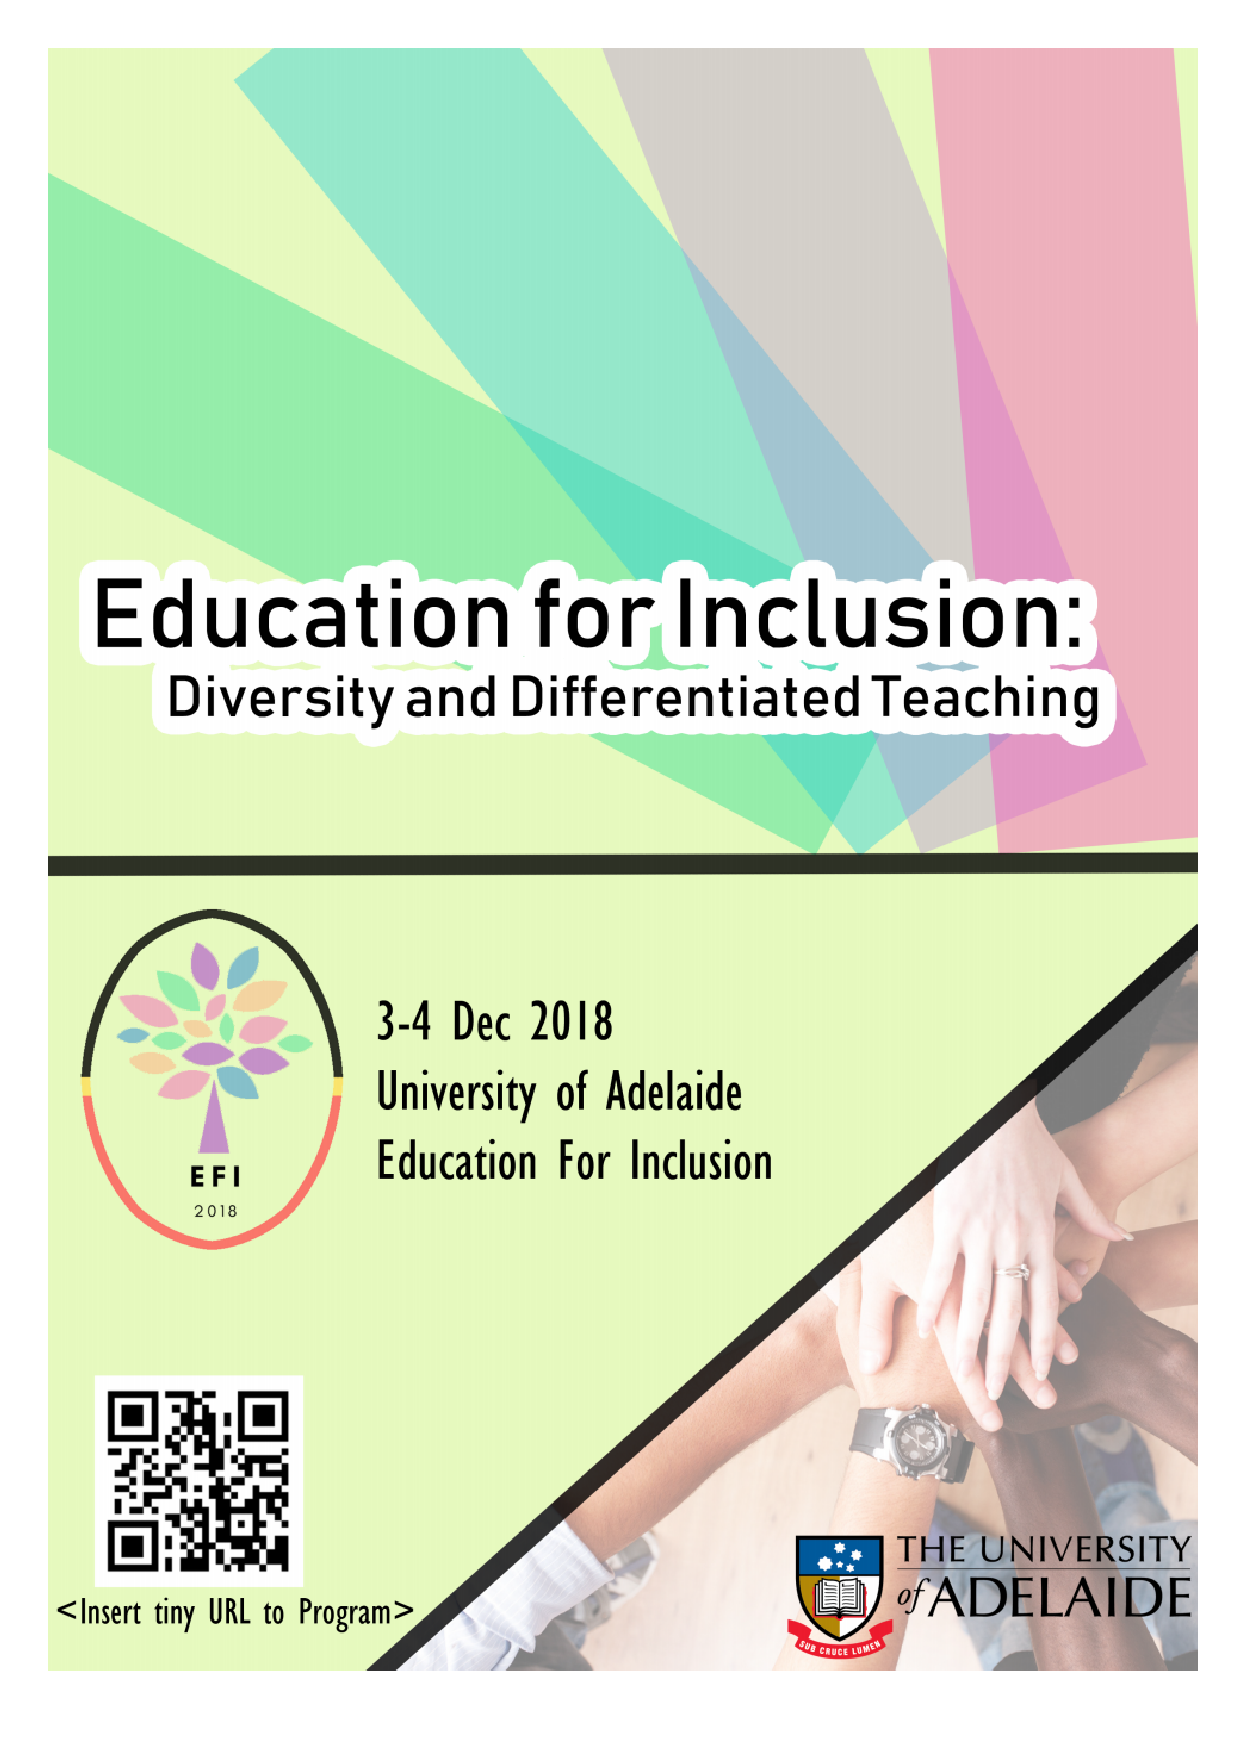
\includepdf[page = 1]{poster.pdf}

% Contents
\tableofcontents
\vfill

% Acknowledgement of Country
\pagebreak
\vspace*{2cm}
{\Huge Acknowledgement of Country}
\vspace{2cm}
\addcontentsline{toc}{chapter}{Acknowledgement of Country}

We acknowledge and pay our respects to the Kaurna people, the traditional custodians whose ancestral lands we gather on. We acknowledge the deep feelings of attachment and relationship of the Kaurna people to country and we respect and value their past, present and ongoing connection to the land and cultural beliefs.
\vfill

% About the Conference
\pagebreak
\vspace*{2cm}
{\Huge About the Conference}
\vspace{2cm}
\addcontentsline{toc}{chapter}{About the Conference}

\lipsum[1-2]
\vfill

% Program
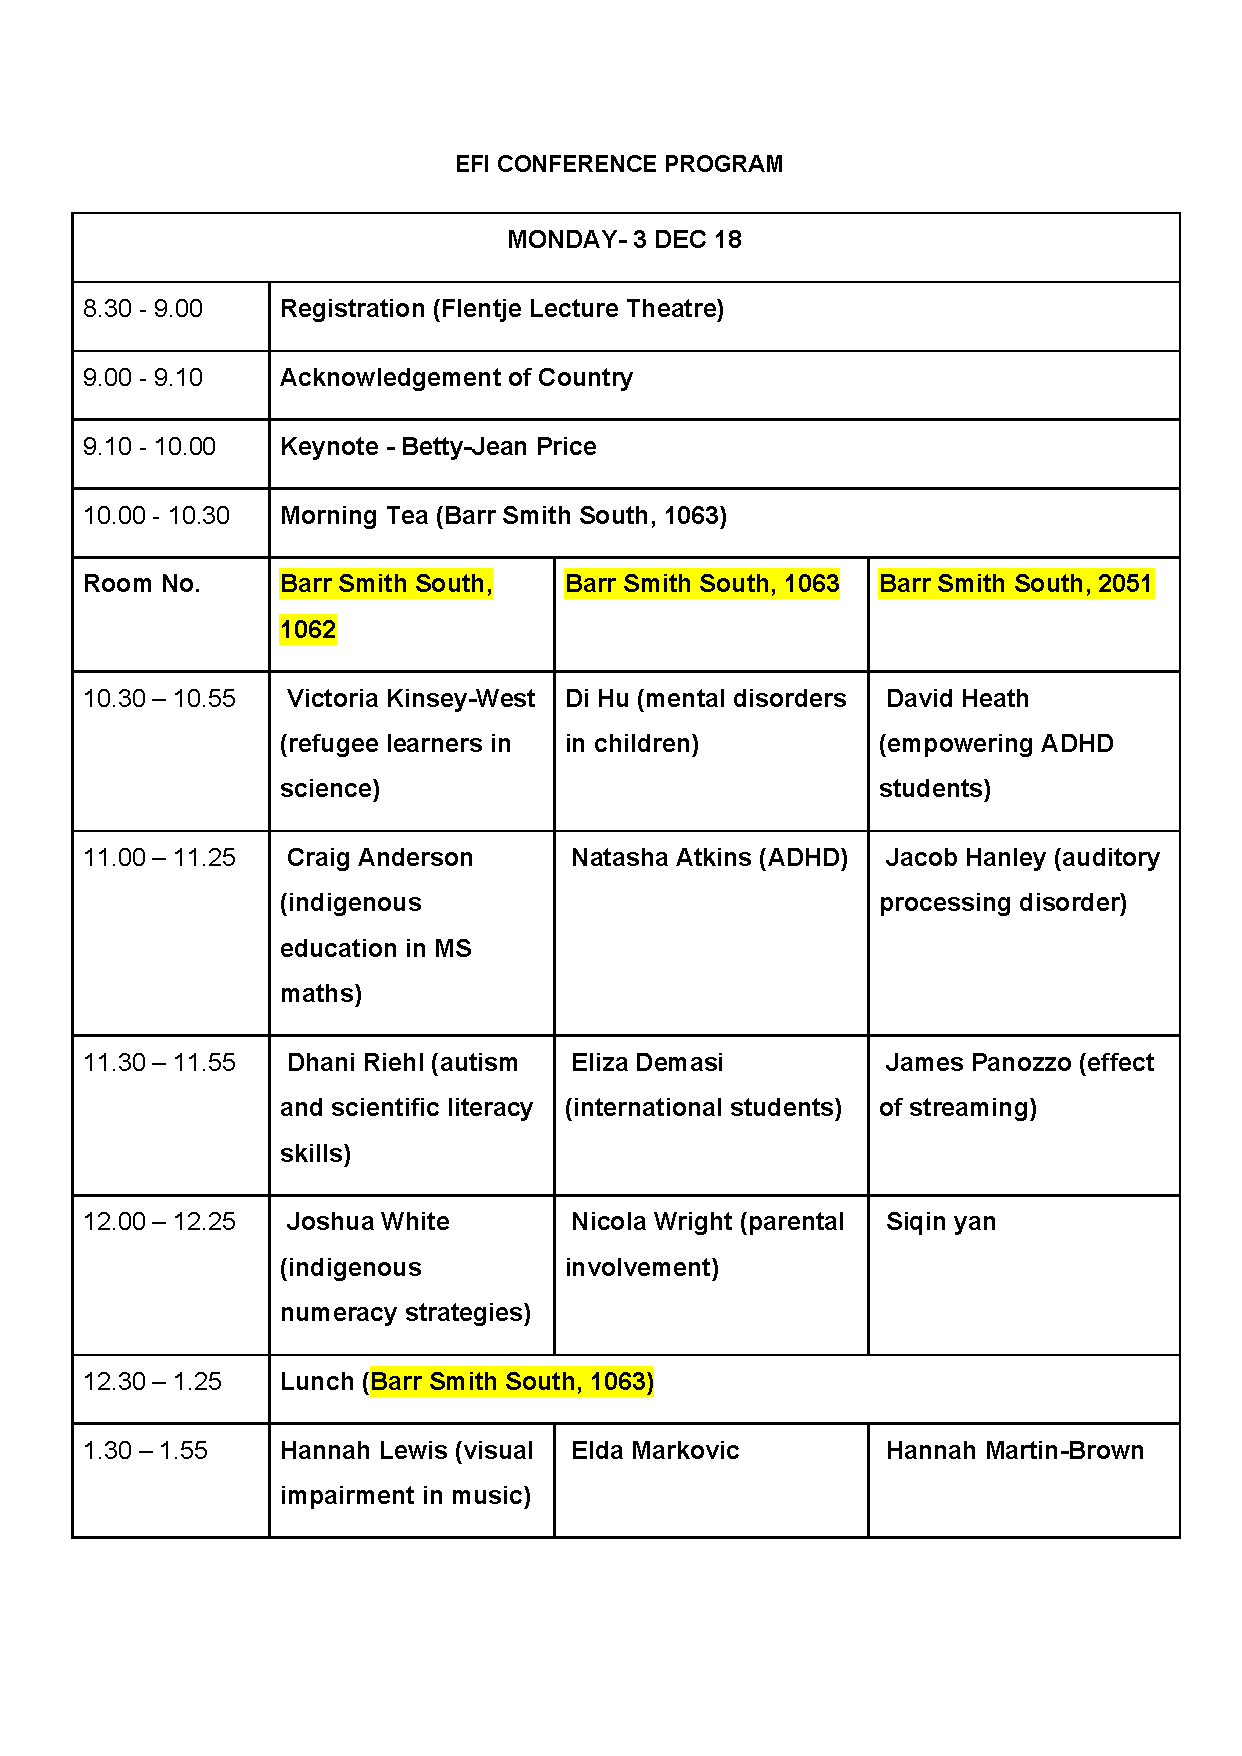
\includepdf[pages = -, addtotoc={1,chapternonum,1,Program,p1}]{program.pdf}

\cleardoublepage

%\renewcommand{\arraystretch}{1.4}
%\begin{sidewaystable}
%\begin{center}
%\begin{tabular}{rcr|p{7cm}|p{7cm}|p{7cm}}
%\multicolumn{4}{c}{MONDAY 3 December 2018} \\ \hline
%8.30 & - & 9.00 & \multicolumn{3}{l}{Registration (Flenje Lecture Theatre)} \\ \hline
%9.00 & - & 9.10 & \multicolumn{3}{l}{Acknowledgement of Country} \\ \hline
%9.10 & - & 10.00 & \multicolumn{3}{l}{Keynote Speaker: Betty-Jean Price} \\ \hline
%10.00 & - & 10.30 & \multicolumn{3}{l}{Morning Tea (Barr Smith South 1063)} \\ \hline
% & & & Barr Smith South 1062 & Barr Smith South 1063 & Barr Smith South 2051 \\ \hline
% 10.30 & - & 10.55 & 
% Victoria Kinsey-West (refugee learners in science) & 
% Di Hu (mental disorders in children) &  
% David Heath (empowering ADHD students) \\ \hline
%11.00 & – & 11.25 &
% Craig Anderson (indigenous education in MS maths) &
% Natasha Atkins (ADHD) &
% Jacob Hanley (auditory processing disorder) \\ \hline
%11.30 & – & 11.55 &
% Dhani Riehl (autism and scientific literacy skills) &
% Eliza Demasi (international students) &
% James Panozzo (effect of streaming) \\ \hline
%12.00 & – & 12.25 &
% Joshua White (indigenous numeracy strategies) &
% Nicola Wright (parental involvement) &
% Siqin yan \\ \hline
%12.30 & - & 1.25 & \multicolumn{3}{l}{Lumch (Barr Smith South, 1063} \\ \hline
%1.30 & – & 1.55 &
% Hannah Lewis (visual impairment in music) &
% Elda Markovic &
% Hannah Martin-Brown \\ \hline
%2.00 & – & 2.25 &
% Vinh-Huy Hua (ADHD) &
% Edward Bonner &
% Yilun Huang \\ \hline
%2.30 & – & 2.55 &
% Betula Barritt &
% Lewis Hodkinson &
% Lyron Winderbaum (indigenous - culture and linguistics maths) \\ \hline
%\end{tabular}
%\end{center}
%\end{sidewaystable}





\chapter*{Abstracts and Biographies}
\addcontentsline{toc}{chapter}{Abstracts and Biographies}

\section*{Keynote Speaker}
\addcontentsline{toc}{section}{Keynote Speaker}


\section*{Michael Cobung}
\addcontentsline{toc}{section}{Michael Cobung}



\pagebreak
\section*{Pre-Service Teacher Presentations}
\addcontentsline{toc}{section}{Pre-Service Teachers}




\subsection*{Effective Indigenisation of Middle School Mathematics While Negating Tokenism, Coiunteracting Anxiety, and Eliminating Prejudice (Craig Anderson)}

In the decade after 2006, Australian school students’ performance rankings – mathematics in particular - have dropped in relation to other OECD nations. Furthermore, in accordance the 2017 SACE enrolment records, much to the discontent of Australian Chief Scientist Alan Finkel, the enrolments in specialist mathematics is significantly lower than the enrolments in physics, and chemistry; subjects were specialist mathematics is required at the university level.
 
It is evident that modern day school students walk a fine line between success and failure within mathematics. The addition of ‘irrelevant’ - or tokenistic - content to an already declining subject does little to alleviate anxiety amongst students. Furthermore, one might argue that tokenism in fact increase prejudice to an already poorly represented culture.
 
More alarmingly, the prejudice exists at the federal level as seen with the 2018 federal liberal leader candidate Peter Dutton, and former liberal shadow minister Sophie Mirabella boycotting the 2008 Rudd Sorry Speech. Furthermore, such recalcitrant views are further compounded by former prime minister - and at the time leader of the opposition - Tony Abbott’s insensitive comments about the Aboriginal Tent Embassy in Canberra. It seems farcical to imagine that any positive change could occur with xenophobic legislators.
 
In a modern era, this presentation explores 1) the nexus between mathematics and culture, 2) the relevance of indigenous content within mathematics, and 3) the usage of culture to counteract anxiety within mathematics. By the end of this presentation, the goal is to commence a pragmatic dialogue on how to equip students with the necessary skills to operate both intelligently and compassionately in an ever-changing technology era.

\subsection*{Craig Anderson}

Craig was awarded a Bachelor of Engineering, Computer Engineering, Honors Class II Division 1 from University of Wollongong in June of 2012.

Afterwards, Craig moved to Melbourne where he worked as an engineer specialising in electronics circuit design, embedded firmware development, production, and equipment service \& repair.

In his spare time, Craig enjoys tinkering with his robots, loitering at his favourite café, and relishing the fact that he no longer works in dungeons.




\subsection*{Attention Deficit Hyperactivity Disorder (ADHD) in a Secondary Classroom (Natasha Atkins)}

The Australian Guidelines on Attention Deficit Hyperactivity Disorder (ADHD) (2009) state that 5-10\% of children and adolescents are diagnosed with ADHD, yet throughout education there seems to be a lack of well-known and easily employable strategies to aid these students at a secondary level. It is recognised that students with ADHD often experience social and academic problems in the classroom (Lessing \& Wulfsohn, 2015) and this research aims to explore and expand on common strategies that are more prominent in primary classrooms and adapt them for use in a secondary space.

ADHD, previously known as Attention Deficit Disorder (ADD) is a neurodevelopmental disorder with a recognised and persistent pattern of behaviour. ADHD begins at birth, for both sexes, and will usually continue through all of life to some degree. ADHD is generally divided into three subcategories: inattentive, hyperactive/impulsive and combined. There is a very large range of symptoms that students with ADHD can show. Typically, students might be easily distracted, forgetful, disruptive and participating in risky, impulsive activities (ADHD Australia), however, educators should realise that the symptoms that each student will display will be different.

DuPaul et. al. (2011) suggest a range of strategies to support students with ADHD overcome their academic difficulties. Some of these strategies include modifying the length or content of assessments, providing students with a choice when asked to complete a task, increasing the use of positive reinforcement and providing more detailed instruction.

It is also important to recognise that students with ADHD can be creative, good public speakers, energetic and enthusiastic (DfE, 2018). Teachers should use each student’s strengths in the classroom to support and encourage their successes. Students with ADHD often have lowered self-esteem because they feel as though they need to work much harder than their peers to complete the same tasks. By incorporating strategies to recognise the positive behaviour of these students, teachers can help lift student’s self-esteem (Child Mind Institute).

Educators need to be aware of a broad range of strategies to incorporate into their secondary planning, lessons and assessments to not only help students with ADHD overcome their difficulties in the classroom, but also to flourish by encouraging the use of their strengths, all while maintaining student self-esteem and inclusion.

\subsection*{Natasha Atkins}

In 2013 Natasha began her tertiary education at the University of Adelaide in a Bachelor of Science (Advanced) which she graduated from in 2015 with a double major in Theoretical and Experimental Physics. In 2016 she began by Masters in Astrophysics and graduated from this in 2018 as well as beginning her journey in Masters of Teaching. 



\subsection*{Supporting students with Autism Spectrum Disorder in a Secondary Music Classroom (Matthew Bailey)}

Within a secondary music classroom, students with Autism Spectrum Disorder (ASD) are at educational risk as a result of not having the necessary support systems in place to meet their needs and requirements. Within ASD, there is a wide range of difficulties that people on the spectrum may face, ranging from high functioning autism (Asperger’s) to nonverbal autism. All people with autism fit on this spectrum differently, thus it is imperative for schools to be able to accommodate both ends of the spectrum. This will be examined through how the Australian Curriculum (ACARA) and South Australian Certificate of Education (SACE) meet the legislative requirements necessary to support these students within a mainstream music classroom. Within this, the curriculum documents will be investigated to determine if there is enough alteration of curricula to provide adequate support for ASD students, particularly focusing on providing opportunities for active participation.
From a legislative standpoint, several documents such as the Disability Discrimination Act (1992) and the subsequent Disability Standards for Education (2005) have been written to support these students. These legislative documents have been examined to identify the scope of support that students with ASD are entitled to in relation to the curricula. In addition, documents such as the Department for Education and Child Development’s ‘Children and Young People Disability Policy’ have been written and appraised, which divides the roles and responsibilities in providing an inclusive education for various levels of authority (e.g. Chief Executive, Teachers, Principals, School Services Officers).
These support systems and legislations require constant communication between schools and parents/carers so that the most effective methods of giving the student an inclusive education. Some of the current methodologies in place include Individual Learning Plans (ILP) and Negotiated Education Plans (NEP), which classroom teachers design in consultation with the parents/carers and school to give their student the necessary support and resources for their education.
The findings of this conference will provide secondary music teachers with strategies to help implement a classroom environment which is inclusive to students with ASD. These strategies will be tailored in accordance with legislative documents and requirements, as well as the SACE and ACARA curriculum documents, whilst also having a focus on the support systems in place which can aid students and teachers with this inclusive method of education.

\subsection*{Matthew Bailey}

Matthew has completed a Bachelor of Music from the Elder Conservatorium of Music, specialising in Jazz Performance. Since then, he has moved into the Masters of Teaching program, specialising in Classroom and Instrumental Music.


\subsection*{Teaching Indigenous Content Respectfully, Sensitively and Confidently in Classroom Music}

\subsection*{Betula Barritt}

Betula has completed a Bachelor of Music (Majoring in Classical Performance) at the Elder Conservatorium of Music. She is a Private Music Instructor on the flute and recorder and has been teaching privately for the past eight years. She looks forward to working in a classroom music setting as well as broadening her experiences as an instrumental teacher through the Masters of Teaching Degree. She has a passion for inclusive teaching and seeks to continue researching and participating in this field.


\subsection*{Edward Bonner}


\subsection*{Beti Boskovic}


\subsection*{Robert Button}


\subsection*{Nick Crowhurst}


\subsection*{Jonathan Daughtry}


\subsection*{Eliza Demasi}


\subsection*{Jacob Hanley}


\subsection*{David Heath}


\subsection*{Lewis Hodkinson}


\subsection*{Elliot Hoskin}


\subsection*{Di Hu}


\subsection*{Vinh-Huy Hua}


\subsection*{Yilun Huang}


\subsection*{Josh Huxtable}


\subsection*{Patrick Johnson}


\subsection*{Victoria Kinsey-West}


\subsection*{Hannah Lewis}


\subsection*{Elda Markovic}


\subsection*{Hannah Martin-Brown}


\subsection*{Kaliese Mcllvena}


\subsection*{James Panozzo}


\subsection*{Dhani Riehl}


\subsection*{Hayley Beth Ruthven}


\subsection*{Robert Spargo}


\subsection*{Kyuseop Suh}


\subsection*{Ting Sun}


\subsection*{Benjamin Tymukas}


\subsection*{Christopher Vogel}


\subsection*{Joshua White}


\subsection*{Lyron Winderbaum}


\subsection*{Nicola Wright}


\subsection*{Siqin Yan}




\end{document}